\chapter{Divisor de potencia Wilkinson}
\label{chap:wilkinson}
\section*{Resumen}

En este capítulo se presenta el diseño y desarrollo de un divisor de potencia Wilkinson de tres puertos. En primer lugar, se analiza el funcionamiento teórico del divisor Wilkinson en los modos par e impar de excitación. Posteriormente, se emplean estos resultados como punto de partida para el diseño del divisor en tecnología microstrip. Finalmente, se presenta el diseño electromagnético, su simulación y optimización, considerando las características del sustrato utilizado y las restricciones de implementación.

\section{Análisis Par-Impar}

Las líneas de un cuarto de longitud de onda ($\lambda/4$) tienen una impedancia característica normalizada $Z$, mientras que la resistencia en derivación (\textit{shunt}) tiene un valor normalizado $r$.

Para el divisor de potencia de reparto igualitario (3~dB), estos valores deben ser: $Z = \sqrt{2}$ y $r = 2$, como se muestra en la Figura~\ref{fig:fig5.1}.

\begin{figure}[H]
    \centering
    \includegraphics[width=0.75\linewidth]{imagenes/Wilkinson.png}
    \caption{(a) Divisor de potencia Wilkinson de división equitativa en microstrip. (b) Circuito equivalente de línea de transmisión. (Fuente: \cite{pozar}).}
    \label{fig:fig5.1}
\end{figure}

Se redibuja el circuito de la Figura~\ref{fig:fig5.1} colocando generadores de tensión en los puertos de salida, como se muestra en la Figura~\ref{fig:fig5.2}. Esta red ha sido dibujada de manera que sea simétrica respecto del plano medio; las dos resistencias de las fuentes, de valor normalizado igual a 2, se combinan en paralelo para dar una resistencia de valor normalizado igual a 1, que representa la impedancia de una fuente adaptada \cite{pozar}.

\begin{figure}[H]
    \centering
    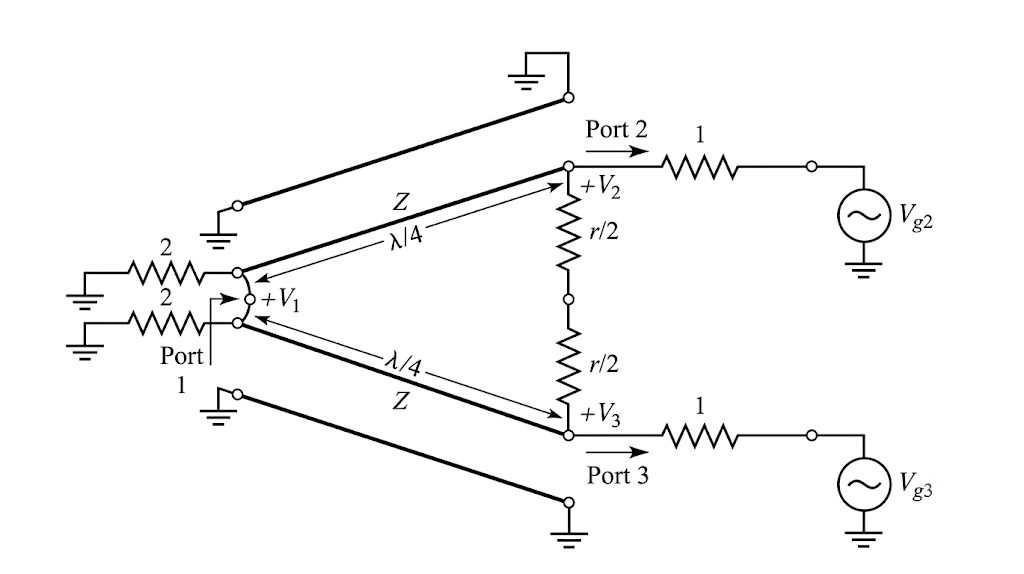
\includegraphics[width=0.75\linewidth]{imagenes/wilkinson dividido.png}
    \caption{Divisor de potencia Wilkinson redibujado de forma simétrica. (Fuente: \cite{pozar}).}
    \label{fig:fig5.2}
\end{figure}

Ahora definimos dos modos distintos de excitación para el circuito de la Figura~\ref{fig:fig5.2}: el modo par, donde $V_{g2} = V_{g3} = 2V_0$, y el modo impar, donde $V_{g2} = -V_{g3} = 2V_0$. La superposición de estos dos modos produce efectivamente una excitación de $V_{g2} = 4V_0$ y $V_{g3} = 0$, a partir de la cual podemos encontrar los parámetros de dispersión de la red. A continuación, analizamos estos dos modos por separado.

\paragraph{Modo par:} Para la excitación en modo par, $V_{g2} = V_{g3} = 2V_0$, por lo que $V_{e2} = V_{e3}$, y por lo tanto no fluye corriente a través de las resistencias de $r/2$ ni por el cortocircuito entre las entradas de las dos líneas de transmisión en el puerto 1. Luego, mirando hacia el puerto 2, vemos una impedancia:
\begin{equation}
Z_{\text{in}}^e = \frac{Z^2}{2}
\label{eq:impedancia_entrada_par}
\end{equation}

ya que la línea de transmisión se comporta como un transformador de cuarto de onda. Por lo tanto, si $Z = \sqrt{2}$, el puerto 2 estará adaptado para la excitación en modo par; entonces $V_{e2} = V_0$ ya que $Z_{\text{in}}^e = 1$. El resistor de $r/2$ resulta superfluo en este caso, ya que un extremo se encuentra en circuito abierto. A continuación, hallamos $V_{e1}$ a partir de las ecuaciones de las líneas de transmisión. Si fijamos $x = 0$ en el puerto 1 y $x = -\lambda/4$ en el puerto 2, podemos escribir el coeficiente de reflexión como:
\begin{equation}
\Gamma = \frac{2 - \sqrt{2}}{2 + \sqrt{2}}
\label{eq:coeficiente_reflexion}
\end{equation}

\paragraph{Modo impar:} Para la excitación en modo impar, $V_{g2} = -V_{g3} = 2V_0$, por lo que $V_{o2} = -V_{o3}$, y existe un nulo de tensión a lo largo del centro del circuito de la Figura~\ref{fig:fig5.2}. Mirando hacia el puerto 2, vemos una impedancia de $r/2$ ya que la línea de transmisión conectada en paralelo tiene una longitud de $\lambda/4$ y está en cortocircuito en el puerto 1, por lo que se comporta como un circuito abierto en el puerto 2. Por lo tanto, el puerto 2 estará adaptado para la excitación en modo impar si seleccionamos $r = 2$. Entonces $V_{o2} = V_0$ y $V_{o1} = 0$; para este modo de excitación toda la potencia se entrega a los resistores de $r/2$, sin que nada de potencia se dirija al puerto 1. 

Finalmente, debemos hallar la impedancia de entrada en el puerto 1 del divisor Wilkinson cuando los puertos 2 y 3 están terminados en cargas adaptadas. Tenemos entonces la conexión en paralelo de dos transformadores de cuarto de onda terminados en cargas de valor unitario (normalizadas). La impedancia de entrada es:
\begin{equation}
Z_{\text{in}} = \frac{1}{2} (\sqrt{2})^2 = 1
\label{eq:zin_wilkinson}
\end{equation}

En resumen, podemos establecer los siguientes parámetros de dispersión para el divisor Wilkinson, expresados en escala lineal \cite{pozar}:

\begin{align*}
S_{11} &= 0 && (Z_{\text{in}} = 1 \text{ en el puerto 1}) \\
S_{22} &= S_{33} = 0 && (\text{puertos 2 y 3 adaptados para los modos par e impar}) \\
S_{12} &= S_{21} = \frac{-j}{\sqrt{2}} && (\text{simetría debido a la reciprocidad}) \\
S_{13} &= S_{31} = \frac{-j}{\sqrt{2}} && (\text{simetría de los puertos 2 y 3}) \\
S_{23} &= S_{32} = 0 && (\text{aislamiento entre los puertos de salida})
\end{align*}
